\RequirePackage{luatex85}
\documentclass[tikz]{standalone}
% Default preamble
\usepackage{pgfplots}
\pgfplotsset{compat=newest}
\usepgfplotslibrary{groupplots}
\usepgfplotslibrary{polar}
\usepgfplotslibrary{smithchart}
\usepgfplotslibrary{statistics}
\usepgfplotslibrary{dateplot}
\usepgfplotslibrary{ternary}
\usepackage[T1]{fontenc}
\usepackage{lmodern}
\begin{document}
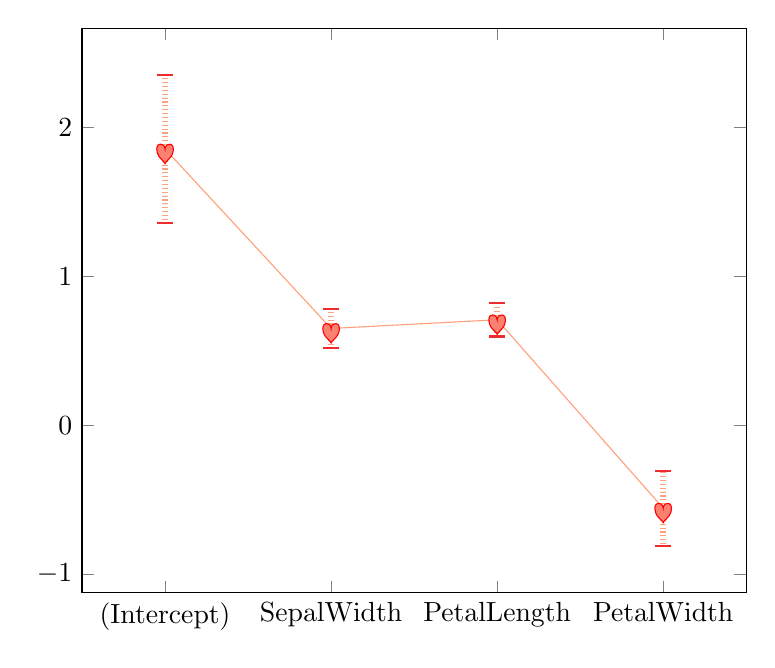
\begin{tikzpicture}
\begin{axis}[title style={}, xlabel style={}, ylabel style={}, xticklabel style={}, yticklabel style={}, width={240pt}, height={204pt}, symbolic x coords={{(}Intercept{)},SepalWidth,PetalLength,PetalWidth}, xtick={{(}Intercept{)},SepalWidth,PetalLength,PetalWidth}, xmin={{[normalized]-0.5}}, xmax={{[normalized]3.5}}, scale only axis]
    \addplot[mark={heart}, mark options={mark size={3pt}, fill={rgb,255: red, 250; green, 128; blue, 114}, fill opacity={1}, draw={rgb,255: red, 255; green, 0; blue, 0}, draw opacity={1}}, error bars/error mark={|}, error bars/error mark options={mark size={3.0pt}, solid, line width={0.8pt}, draw={rgb,255: red, 238; green, 44; blue, 44}, draw opacity={1}}, error bars/error bar style={draw={rgb,255: red, 255; green, 160; blue, 122}, draw opacity={1}, densely dotted, line width={2pt}}, draw={rgb,255: red, 255; green, 160; blue, 122}, draw opacity={1}, error bars/y dir={both}, error bars/y explicit]
        coordinates {
            ({(}Intercept{)},1.8559974929172318) +- (0,0.49562225706654334)
            (SepalWidth,0.6508371593133089) +- (0,0.1317182882857669)
            (PetalLength,0.7091319591367299) +- (0,0.11209691841092581)
            (PetalWidth,-0.5564826601669999) +- (0,0.25207883587827457)
        }
        ;
\end{axis}
\end{tikzpicture}
\end{document}
